\documentclass[fleqn]{article}
\usepackage{amsmath}
\usepackage[dvips]{graphicx}
\bibliographystyle{plain}
%__________________________________
\begin{document}

\section*{\center Colliding Disks}
\subsection*{\underline{Problem Description}}
This is an implementation of an example calculation from \cite{sulskycmame} in
which two elastic disks collide and rebound.  See Section 7.3 of that
manuscript for a description of the problem.
 
\subsection*{\underline{Simulation Specifics}}
\begin{description} 
\item [Component used:] \hfill MPM
\item [Input file name:] \hfill disks_sulsky.ups
\item [Command used to run input file:]\hfill sus disks_sulsky.ups
\item [Simulation Domain:]\hfill    1.0 x 1.0 x 0.05 m

\item [Cell Spacing:]\hfill \\ 
.05 x .05 x .05 m (Level 0)

\item [Example Runtimes:] \hfill \\
 1 minute   (1 processor, 3.0 GHz Xeon)\\

\item [Physical time simulated:] \hfill 3.0 seconds

\item [Associate scirun network:] \hfill disks.srn

\end{description}

\section*{\underline{Results}}

Figure~\ref{figdisks} shows a snapshot of the simulation, as the disks
are beginning to collide.
\begin{figure}[b]
  \center
%  \scalebox{0.2}{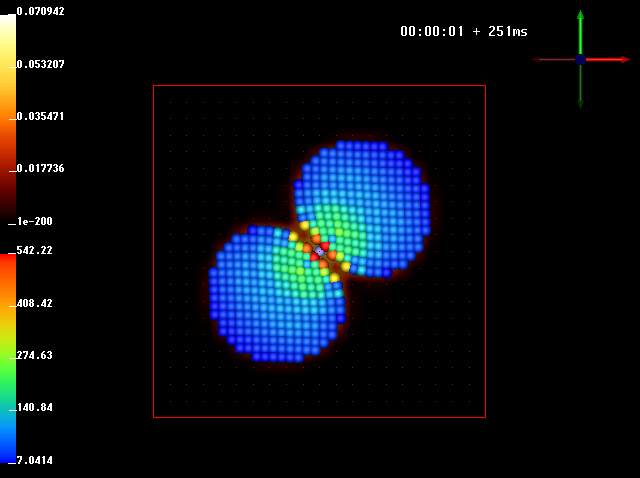
\includegraphics{disks.png}}
  \caption{Colliding elastic disks.  Particles colored according to
equivalent stress, grid according to nodal mass.}
  \label{figdisks}
\end{figure}

Additional data is available within the uda in the form of "dat" files.
In this case, both the kinetic and strain energies are avaiable and can
be plotted to create a graph similar to that in Fig. 5a of \cite{sulskycmame}.
e.g. using gnuplot:

cd disks.uda.000
gnuplot
gnuplot> plot "StrainEnergy.dat", "KineticEnergy.dat"
gnuplot> quit

\bibliography{../references}

\end{document}
